% !TEX root = pfe-book1.tex
%!TEX TS-program = pdflatex
%!TEX encoding = UTF-8 Unicode

\chapter{Pressure}
\section{Hydraulic Press}
A hydraulic press is an ancient machine, but it has retained its significance to the present day. Take a look at \figr{fig-7-01} depicting a hydraulic press. Two pistons -- small and large -- can move in a vessel with water. If we press one piston with our hand, the pressure is transmitted to the other piston -- it will rise. Just as much water will rise above the initial position of the second piston as the first piston presses down into the vessel.
\begin{figure}[!ht]
\centering
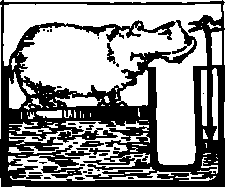
\includegraphics[width=0.65\textwidth]{figures/fig-7-1.pdf}
\caption{A hydraulic press.}
\label{fig-7-01}
\end{figure}


If the areas of the pistons are $S_{1}$ and $S_{2}$ and their displacements are $l_{1}$ and $l_{2}$ the equality of the volumes
yields 
\begin{equation*}%
S_{1} l_{1} = S_{2} l_{2}, \quad \textrm{or} \quad \dfrac{l_{1}}{l_{2}} =\dfrac{S_{2}}{S_{1}} 
\end{equation*}
We must discover the equilibrium condition for the pistons.

We shall find such a condition without difficulty, starting out from the fact that the work performed by the balancing forces should be equal to zero. Then during the displacement of the pistons the works done by the forces exerted on them should be equal (with opposite signs). Therefore,
\begin{equation*}%
F_{1} l_{1} = F_{2} l_{2}, \quad \textrm{or} \quad \dfrac{F_{2}}{F_{1}} =\dfrac{l_{1}}{l_{2}} 
\end{equation*}
Comparing this with the preceding equality, we see that
\begin{equation*}%
\dfrac{F_{2}}{F_{1}} =\dfrac{S_{2}}{S_{1}} 
\end{equation*}
This equation implies the possibility of an enormous
multiplication of force. The piston transmitting pressure
can have an area which is hundreds or thousands of
times smaller. The force acting on the large piston will
be just as many times greater compared to the muscular
force.

With the aid of a hydraulic press, one can forge and
punch metals, press the juice out of grapes and raise
weights.

Of course, the gain in force will be accompanied by a loss in path. In order to compress a body by \SI{1}{\centi\meter} with a press, one's hand would have to cover a path as many times greater as the forces $F_{2}$ and $F_{1}$ differ.

Physicists call the ratio of the force to the area, $F/S$, the \emph{pressure} (it is denoted by the letter $p$). Instead of saying, ``One kilogram-force acts on an area of  \SI{1}{\centi\meter\squared} we shall say more concisely, ``The pressure $p = \SI{1}{\kgf\per\centi\meter\squared}$.'' This pressure is called the technical atmosphere (\SI{1}{\kgf\per\centi\meter\squared} = \SI{1}{\atmos}).

Instead of the relation 
\begin{equation*}%
\dfrac{F_{2}}{F_{1}} =\dfrac{S_{2}}{S_{1}},
\end{equation*}
one can now write:
\begin{equation*}%
\dfrac{F_{2}}{S_{2}} =\dfrac{F_{1}}{S_{1}}, \quad \textrm{i.e.} \quad p_{1}=p_{2}
\end{equation*}
Thus, the pressures on both the pistons are the same. Our reasoning does not depend on where the pistons are located or whether their surfaces are horizontal, vertical or inclined. And in general, it is not a matter of pistons. One may conceptually choose any two portions of a surface enclosing a liquid, and assert that the pressures on them are identical.

It turns out, therefore, that the pressure within a liquid is the same at all its points and in all the directions. In other words, an identical force is exerted on area elements of a definite size, irrespective of their orientation. This fact is called \emph{Pascal's law}.

\section{Hydrostatic Pressure}
Pascal's law is valid for liquids and gases. However, it fails to take into account an important circumstance -- the existence of weight.

Under terrestrial conditions, this should not be forgotten. Even water has weight. It is therefore obvious that two area elements situated at different depths under water will experience different pressures. But what will this difference be equal to? Let us conceptually single out within a liquid a right cylinder with horizontal bases. The water inside it presses on the surrounding
water. The resultant force of this pressure is equal to the weight $mg$ of the liquid in the cylinder \figr{fig-7-02}. This resultant force is made up of the forces acting on the bases of the cylinder and on its lateral surface. But the forces acting on opposite sides of the lateral surface are equal in magnitude and opposite in direction. Therefore, the sum of all the forces acting on the lateral surface
is equal to zero. Hence, the weight $mg$ will be equal to the difference in force, $F_{2} - F_{1}$. If the height of the
cylinder is $h$, the area of its base is $S$, and the density
of the liquid is $\rho$, we may write $\rho g h S$ instead of $mg$.

\begin{figure}[!ht]
\centering
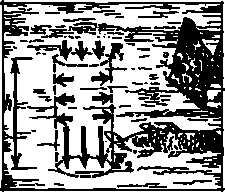
\includegraphics[width=0.65\textwidth]{figures/fig-7-2.pdf}
\caption{Hydrostatic pressure on a column of water.}
\label{fig-7-02}
\end{figure}


The difference in force is equal to this quantity. In order to obtain the difference in pressure, we must divide the
weight by the area $S$. The difference in pressure turns out equal to $\rho gh$.

In accordance with Pascal's law, the pressure on differently oriented area elements located at the same depth will be identical. Hence, at two points of a liquid situated one above the other at height $h$ the difference in pressure will equal the weight of a column of the liquid whose cross-sectional area is equal to unity and whose height is $h$:
\begin{equation*}%
p_{2} - p_{1} = \rho gh
\end{equation*}
A pressure exerted by water caused by its weight is called \emph{hydrostatic}.

Under terrestrial conditions, air most often presses down on the free surface of a liquid. The pressure exerted by air is called \emph{atmospheric}. The pressure at a depth is composed of atmospheric and hydrostatic pressures.

In order to compute the force due to water pressure, it is only necessary to know the size of the area element on which it is exerted and the height of the column of liquid above it. By virtue of Pascal's law, nothing else plays any role.

\begin{figure}[!ht]
\centering
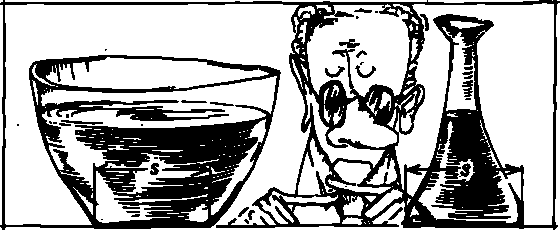
\includegraphics[width=0.85\textwidth]{figures/fig-7-3.pdf}
\caption{Are the forces at the bottom of the two vessels same?}
\label{fig-7-3}
\end{figure}


This may seem surprising. Is it possible for the forces acting on the identical bottoms of the two vessels depicted \figr{fig-7-3} to be the same? Indeed, there is much more water in the vessel on the left. In spite of this, the forces acting on the bottoms are equal to $\rho g h S$ in both cases. This is greater than the weight of the water in the vessel on the right and less than the weight of the water in the vessel on the left. The sloping walls of the vessel on the left support the weight of the ``extra'' water, but on the right, on the contrary, they add reaction forces to the weight of the water. This interesting phenomenon is sometimes called the hydrostatic paradox.

If two vessels of different form, but with water at the same level, are connected by means of a tube, water will not flow from one vessel to another. Such a flow could take place in case the pressures in the vessels were different. But this is not the case, and so the liquid in communicating vessels will always stand at one and the same level regardless of their form.

On the contrary, if the water levels in communicating vessels are different, water will begin moving and the levels will equalize.

Water pressure is much greater than air pressure. At a depth of \SI{10}{\meter}, water pressure is twice atmospheric pressure, at a depth of \SI{1}{\kilo\meter}, it is equal to \SI{100}{\atmos}.

Oceans have depths greater than \SI{10}{\kilo\meter} at certain places. The forces due to water pressure at such depths are exceptionally great. Pieces of wood which are lowered to a depth of \SI{5}{\kilo\meter} are so compressed by this enormous pressure that, after such a ``baptism'', they sink like bricks in a barrel of water.

This enormous pressure makes great difficulties for investigators of marine life. Deep-sea descents are carried out in steel globes -- the so-called bathyspheres or bathyscaphes -- which have to withstand pressures greater than \SI{1000}{\atmos}.

But submarines can dive to a depth of only \SIrange{100}{200}{\meter}.

\section{Atmospheric Pressure}

We live on the bottom of an ocean of air -- the atmosphere. Each body, every grain of sand, any object situated on the Earth is subject to air pressure.

Atmospheric pressure isn't so small. A force of about \SI{1}{\kgf} acts on each square centimetre of a body's surface. The cause of atmospheric pressure is obvious. Just as water, air possesses weight and, therefore, exerts a pressure equal (just as for water) to the weight of the column of air above the body. The higher we climb up a mountain, the less air there will be above us and, therefore, the lower will atmospheric pressure become. One must know how to measure pressure for scientific
and everyday purposes. There exist special instrument -- \emph{barometers} -- for this.

It isn't difficult to make a barometer. Mercury is poured into a tube with one end sealed off. Closing the open end with a finger, one turns the tube upside-down and submerges its open end in a cup of mercury. When this is done, the mercury in the tube will fall, but will not all pour out. The space above the mercury in the tube is undoubtedly airless. The mercury is supported in the tube by the pressure of the external air \figr{fig-7-4}.


\begin{figure}[!ht]
\centering
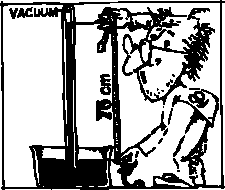
\includegraphics[width=0.65\textwidth]{figures/fig-7-4.pdf}
\caption{A barometer.}
\label{fig-7-4}
\end{figure}


Whatever the dimensions of the cup with mercury, and whatever the diameter of the tube, the mercury will stand at about one and the same height -- \SI{76}{\centi\meter}.

If we take a tube shorter than \SI{76}{\centi\meter}, it will be completely filled by mercury and we will not see any vacuum. A \SI{76}{\centi\meter} column of mercury presses down on the support with the same force as the atmosphere. This mercury column with a cross-sectional area of \SI{1}{\centi\meter\squared} presses down with a force of
\SI{1.033}{\kgf}. This number is the volume of the mercury $1 \times \SI{76}{\centi\meter\cubed}$ multiplied by its density and the acceleration of free fall.

As you see, the average atmospheric pressure (usually called standard atmospheric pressure) that is exerted on everything on the Earth is close to the pressure that \SI{1}{\kilo\gram} weight exerts on an area of \SI{1}{\centi\meter\squared}.

Various units are used in measuring pressures. One often simply indicates the height of a mercury column in millimetres. For example, we say that the pressure is above normal today, it is equal to \SI{768}{\milli\meter\mercury} (i.e. of mercury).

A pressure of \SI{760}{\milli\meter\mercury} is sometimes called a \emph{standard atmosphere}. A pressure of \SI{1}{\kgf\per\centi\meter\squared} is called a \emph{technical atmosphere}. Since the difference between a physical
atmosphere and a technical atmosphere is very small, from now on we will not distinguish between them.

Physicists also make frequent use of another unit of pressure, the \emph{bar}; 
\begin{equation*}%
\SI{1}{\bar} =\SI{d6}{\dyne\per\centi\meter\squared}
\end{equation*}
 Since \SI{1}{\gf} = \SI{981}{\dyne}, one bar is approximately equal to one atmosphere. More precisely, standard (normal) atmospheric pressure roughly equals 1013 millibars.
 
The unit of pressure in the SI system is the \emph{pascal} (\si{\pascal}), which is the pressure produced by a force of \SI{1}{\newton} acting on an area of \SI{1}{\meter\squared}. This is very little pressure, as can be seen from the fact that 
\begin{equation*}%
\SI{1}{\pascal} = \SI{1}{\newton\per\metre\squared} = 10\,\,\textrm{dyn}/ \si{\centi\metre\squared} = 10^{-5}\,\, \textrm{bar}.
\end{equation*}
Computing the area of the Earth's surface with the aid of the formula $4 \pi R^{2}$ , we find that the weight of the entire atmosphere is expressed by the enormous figure of \SI{5d18}{\kgf}.

Barometer tubes can have the most varied forms; only one thing is important: one of the ends of the tube must be sealed off in such a way that there be no air above the surface of the mercury. Atmospheric pressure acts on the other level of the mercury.

Atmospheric pressure can be measured by a mercury
barometer with a very great accuracy. Of course, it isn't
necessary to use only mercury; any other liquid is suitable.
But mercury is the heaviest liquid, and so the height
of a mercury column under standard pressure will be
minimum. The mercury barometer is not a particularly
convenient instrument. It is not good to leave a surface
of mercury open (mercury vapour is poisonous); further-
more, this instrument is not portable.

These drawbacks are not shared by aneroid barometers -- aneroids (i.e. airless). Everyone has seen such a barometer. It is a small round metal box with a scale and a pointer. Values of pressure are marked on the scale, usually in centimetres of a mercury column. The air has been pumped out of the metal box. The cover of the box is kept in place by a strong spring, since it would otherwise be crushed by atmospheric pressure.

\begin{figure}[!ht]
\centering
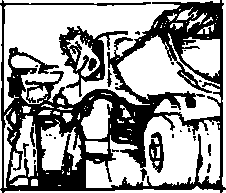
\includegraphics[width=0.65\textwidth]{figures/fig-7-5.pdf}
\caption{A siphon used to transfer liquids.}
\label{fig-7-5}
\end{figure}

With a change in atmospheric pressure, the cover either
bends or straightens. The pointer is connected to the cover
in such a manner that the pointer moves to the right
when the cover is bent.

Such a barometer is graduated by comparing its readings with those of a mercury barometer. If you want to know the pressure, don't forget to knock on the barometer with your finger. The pointer of the dial experiences considerable friction and usually gets stuck at ``yesterday's weather''.

A simple mechanism -- the siphon -- is based on atmospheric pressure,

A driver wants to help his friend, who is out of gas. But how can gasoline be poured from the tank of his car? It can't be inclined like a tea-kettle.

A rubber tube comes to his aid. He lowers one of its ends into his gas tank and orally sucks the air out of the other end. Then a rapid motion-the open end is stopped up with a finger and placed at a height below the gas tank. Now the finger can be removed -- the gasoline will pour out of the hose \figr{fig-7-5}.

A bent rubber tube is just what a siphon is. The liquid moves in this case for the same reason as through a straight inclined tube. In the final analysis, the liquid flows downwards in both cases.

Atmospheric pressure is necessary for the action of
a siphon: it ``props up'' the liquid and doesn't let the
column of liquid in the tube break. If there were no
atmospheric pressure, the column would break at the
transfer point and the liquid would slip into both vessels.

The siphon starts functioning when the liquid in the
right-hand (i.e. the ``pouring'') part of the tube drops
below the level of the liquid being siphoned off, into
which the left end of the tube has been lowered. The
liquid would otherwise flow back.

\section{How Atmospheric Pressure Was Discovered}

Suction pumps were already known to ancient civilizations. Water could be raised to a considerable height with their aid. Water very obediently followed the piston of such a pump.

Ancient philosophers thought about the causes for this and arrived at the following profound conclusion: water follows the piston because nature fears a vacuum and so does not leave any free space between the piston and the water.

It is told that an artisan constructed for the Duke of Tuscany in Florence a suction pump whose piston was supposed to draw water to a height of more than \SI{10}{\meter}. But no matter how they tried to begin sucking up water with this pump, nothing came of it. The water rose \SI{10}{\meter} with the piston, but after that the piston left the water behind, and so the very same vacuum which nature fears was formed. 

When Galileo was asked to explain the cause of this failure, he answered that nature really dislikes a vacuum, but only up to a certain point. A disciple of Galileo, Evangelista Torricelli (1608-1647), evidently used this case as an excuse to perform his famous experiment in 1643 with a tube filled with mercury. We have just described this experiment -- the constructing of a mercury barometer is precisely Torricelli's experiment.

Taking a tube of height more than \SI{76}{\centi\meter}, Torricelli created a vacuum over the mercury (it is often called a \emph{Torricellian vacuum} in his honour) and thus proved the existence of atmospheric pressure.

By means of this experiment, Torricelli cleared up the misunderstanding of the Duke of Tuscany's artisan. In fact, it is easy to see how many metres water will humbly follow the piston of a suction pump. This motion will continue until the column of water with an area of \SI{1}{\centi\meter\squared} acquires a weight of \SI{1}{\kgf}. Such a column of water will have a height of \SI{10}{\meter}. This is why nature fears a vacuum \ldots{}, but only up to \SI{10}{\meter}.

In 1654, 11 years after Torricelli's discovery, the
action of atmospheric pressure was graphically demonstrated by the Burgomaster of Magdeburg, Otto von Guericke (1602-1686). It wasn't so much the physical essence of the experiment as the theatricality of its performance that brought the author renown.

Two copper hemispheres were connected by an annular
washer. The air was pumped out of the sphere so obtained
through a pipe attached to one of the hemispheres, after
which it was impossible to separate the hemispheres.
A detailed description of Guericke's experiment has been
preserved. The atmospheric pressure on the hemispheres
can now be calculated: for a diameter of \SI{37}{\centi\meter}, the force was approximately equal to \SI{1000}{\kgf}. In order to separate
the hemispheres, Guericke ordered that two teams of
eight horses each be harnessed. Ropes passing through
the rings attached to the hemispheres were tied to the
harnesses. The horses proved unable to separate the
Magdeburg hemispheres.

The forces supplied by eight horses (exactly eight and not sixteen, since the second team harnessed for greater effect could have been replaced by a hook nailed to the wall, with no change in the force acting on the hemispheres) were not enough to break the Magdeburg hemispheres.

If there is a cavity between two bodies in contact, these bodies will not come apart because of atmospheric pressure.

\section{Atmospheric Pressure and Weather}

Pressure fluctuations caused by the weather are very
irregular. At one time people thought that pressure
alone determines the weather. Therefore, the following
inscriptions have been placed on barometers up to the
present day: clear, dry, rain, storm. You can even find
the inscription ``earthquake''.

Changes in pressure really do playa big role in changing the weather. But this role is not decisive. Average or
standard pressure at sea level is equal to 1013~millibars. Pressure fluctuations are comparatively small. The pressure rarely falls below 935-940 millibars or rises to 1055-1060. The lowest pressure -- 885 millibars -- was registered on August 18, 1927, in the South China Sea. The highest -- about 1080 millibars -- was registered on January 23, 1900, at the Barnaul station in Siberia (all figures are taken with respect to sea level).



A map used by meteorologists analyzing changes in the weather is depicted on next page \figr{fig-7-6}. The lines drawn
on the map are called isobars. The pressure is the same along each such line (its value is indicated). Note the regions of the lowest and highest pressures -- the pressure ``peaks'' and ``pockets''. The directions and strengths of winds are related to the distribution of atmospheric pressure. 

Pressures are not identical at different places on the Earth's surface, and a higher pressure ``squeezes'' air into places with a lower pressure. It would seem that a wind should blow in a direction perpendicular to the isobars, i.e. where the pressure is falling most rapidly. However, wind maps show otherwise. The Coriolis force interferes with air pressure and contributes corrections which are
very significant.


\begin{figure}[!ht]
\centering
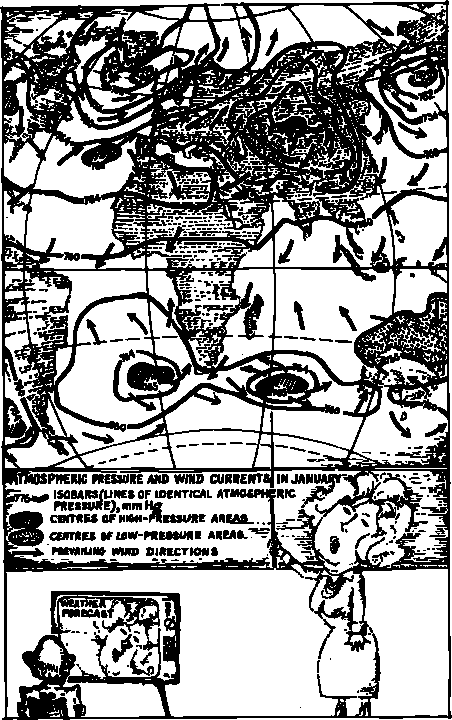
\includegraphics[width=0.75\textwidth]{figures/fig-7-6.pdf}
\caption{A map for weather forecasting showing isobars.}
\label{fig-7-6}
\end{figure}


As we know, a Coriolis force directed to the right of the motion acts on any body moving in the Northern Hemisphere. This also pertains to air particles. ``Squeezed out'' of places of higher pressure and into places where the pressure is lower, the particle should move across the isobar, but the Coriolis force deflects it to the right, and so the direction of the wind forms an angle of about \ang{45} with the direction of the isobar.

A strikingly large effect for such a small force! This is explained by the fact that the obstacles to the action of the Coriolis force -- the friction between layers of air -- are also very insignificant.

The influence of the Coriolis force on the direction of winds at pressure ``peaks'' and ``pockets'' is even more interesting. Owing to the action of the Coriolis force, the air leaving a pressure ``peak'' does not flow in all directions along radii, but moves along curved lines -- spirals. These spiral air streams twist in one and the same direction and create a circular whirlwind displacing air masses clockwise in a high-pressure area. \figr{fig-2.16} clearly shows how a radial motion is converted into a spiral motion under the action of a constant deflecting force (see p.~\pageref{fig-2.16}).

The same thing also happens in a low-pressure area. In the absence of the Coriolis force, the air would flow towards this area uniformly along all radii. However, along the way air masses are deflected to the right. In this case, as is clear from the figure, a circular whirlwind is formed moving the air counterclockwise.

Winds in low-pressure areas are called \emph{cyclones}; winds in high-pressure areas are called \emph{anticyclones}. 

You shouldn't think that every cyclone implies a hurricane or a storm. The passing of cyclones or anticyclones through the city where we live is an ordinary phenomenon related, it is true, more often than not to a change in weather. In many cases, the approach of a cyclone means the coming of bad weather, while the approach of an anticyclone the coming of good weather. 

Incidentally, we shall not embark on the path of a weather forecaster.

\section{Change of Pressure with Altitude}

Pressure falls with an increase in altitude. This was first clarified by the Frenchman Florin P\'erier in 1648 on the instructions of Blaise Pascal. Mt. Puy de Dome, near where P\'erier lived, was \SI{975}{\meter} high. Measurements showed that the mercury in a Torricellian tube falls by \SI{8}{\milli\meter} when this mountain is climbed.


A fall in air pressure with an increase in altitude is
quite natural, for a smaller column of air then presses
down on the instrument.

If you have ever flown in an airplane, you should know
that there is an instrument on the front wall of the cabin
indicating the altitude of the airplane with an accuracy
to within tens of metres. This instrument is called an
altimeter. This is an ordinary barometer, but it has been
calibrated to show heights above sea level.

Pressure falls with an increase in altitude; let us find
a formula of this dependence. We single out a small
layer of air with an area of \SI{1}{\centi\meter\squared}  located between altitudes $h_{1}$ and $h_{2}$. The change of density with altitude is hardly noticeable within a layer which is not too large. Therefore, the weight of the volume of air we have singled
out (it is a small cylinder of height $h_{2} - h_{1}$ and base area of \SI{1}{\centi\meter\squared}) will be
\begin{equation*}%
mg = \rho \, (h_{2} - h_{1}) \, g
\end{equation*}
This weight is just what yields the fall in pressure caused by rising from altitude $h_{1}$ to altitude $h_{2}$, that is
\begin{equation*}%
\dfrac{p_{1} - p_{2}}{\rho} = g \, (h_{2} - h_{1}) 
\end{equation*}
But according to Boyle's law, which should be known to the reader (and if not, he will find it in the second book, p.~33), the density of a gas is proportional to its pressure. Consequently,
\begin{equation*}%
\dfrac{p_{1} - p_{2}}{p} \propto  (h_{2} - h_{1}) 
\end{equation*}

On the left is the fraction by which the pressure grew when the altitude was lowered from $h_{2}$ to $h_{1}$. Hence, a growth in pressure by one and the same percent will correspond to identical drops of $h_{2} - h_{1}$.

Measurements and calculations in complete agreement with each other show that the pressure will fall by 0.1 of its value for each kilometre rise above sea level. The same also holds for descents into deep shafts under sea level -- the pressure will increase by 0.1 of its value when we descend by one kilometre.

We are talking about a change of 0.1 from the value at the previous altitude. This means that during an ascent of \SI{1}{\kilo\meter}, the pressure decreases to 0.9 of the pressure at sea level; during an ascent through the next kilometre, it will become equal to 0.9 of 0.9 of the pressure at sea level; at an altitude of  \SI{3}{\kilo\meter}, the pressure will be equal to 0.9 of 0.9 of 0.9, i.e. $0.9^{3}$ , of the pressure at sea level. It is not difficult to continue this reasoning further.

Denoting the pressure at sea level by $p_{0}$, we can write out the pressure at altitude $h$ (expressed in kilometres):
\begin{equation*}%
p = p_{0} (0.87)^{h} = p_{0} \times 10^{-0.06h} 
\end{equation*}
A more precise number is written in parentheses: 0.9 is the rounded-off value. The formula presupposes the
identical temperature at all altitudes. But as a matter of fact, the temperature of the atmosphere changes with
altitude and does so, moreover, in accordance with a rather complicated law. Nevertheless, the formula
yields fairly good results and may be used for altitudes up to hundreds of kilometres.

It is not hard to determine with the aid of this formula that on the top of the Elbrus -- about \SI{5.6}{\kilo\meter} -- the pressure will fall by a factor of approximately two, while at an altitude of \SI{22}{\kilo\meter} (the record height of a stratospheric balloon's ascent with people), the pressure will fall to \SI{50}{\milli\meter\mercury}.

When we say that a pressure of  \SI{760}{\milli\meter\mercury} is standard, we must not forget to add, ``at sea level''. At an altitude
of  \SI{5.6}{\kilo\meter}, the standard pressure will not be 760, but  \SI{380}{\milli\meter\mercury}.

Along with pressure, air density also falls with an increase in altitude according to the same law. At an altitude of \SI{160}{\kilo\meter}, not much air will remain.

In fact,
\begin{equation*}%
(0.87)^{160} = 10^{-10} 
\end{equation*}

The air density at the Earth's surface is equal to about  \SI{1000}{\gram\per\centi\metre\cubed}, which means that according to our formula there should be \SI{d-7}{\gram} of air in  \SI{1}{\metre\cubed} at an altitude of \SI{160}{\kilo\meter}. But in reality, as measurements performed with the aid of rockets show, the air density at this height is ten times as great.

Our formula gives us an even greater underestimation for heights of several hundreds of kilometres. The change of temperature with altitude and also a particular phenomenon -- the decay of air molecules under the action of solar radiation -- are responsible for the fact that the formula becomes useless at great heights. Here we shall not go into this.

\section{Archimedes' Principle}

Let us hang a weight on a spring balance. The spring will stretch and show how much the weight weighs. Without taking the weight off the spring balance, let us submerge it in water. Will the reading of the spring balance change? Yes, the weight of the body seems to decrease. If the experiment is done with an iron kilogram weight, the ``loss'' in weight will constitute approximately
140~grams.

But what is the matter? For it is clear that neither mass of the weight nor its attraction by the Earth could have changed. There can be only one cause of the loss in weight: an upward force of 140~gf acts on the weight submerged in water. But where does this buoyant force discovered by the great scientist of antiquity, Archimedes, come from? Before considering a solid body in water, let
us consider ``water in water''. We conceptually single out an arbitrary volume of water. This volume possesses
weight, but does not fall to the bottom. Why? The answer is obvious -- the hydrostatic pressure of the surrounding water prevents this. This implies that the resultant of this pressure in the volume under consideration is equal to the weight of the water and directed vertically upwards.

If this volume is now occupied by a solid body, it is clear that the hydrostatic pressure will remain the same.

Thus, as a result of hydrostatic pressure, a force acts on a body immersed in a fluid. The force is directed vertically upwards and is equal in magnitude to the weight of the fluid displaced by the body. This is \emph{Archimedes' principle}.

It is said that Archimedes lay in a bath-tub and thought about how to determine whether or not there is any silver in a gold crown. A person taking a bath distinctly feels a buoyant force. Suddenly the principle came to light, presented itself to Archimedes in its remarkable simplicity. With a cry of  ``Eureka!'' (which means ``I found it!''), Archimedes jumped out of the bath-tub and ran into
the room containing the precious crown in order to immediately determine its loss of weight in water.

The loss of weight of a body in water will be equal to the weight of the water displaced by the body. Knowing the weight of the water, we shall immediately determine its volume, which is equal to the volume of the crown. Knowing the weight of the crown, we can immediately find the density of the material out of which it was made and, knowing the density of gold and silver, find the fraction of silver in the crowd.

\begin{figure}[!ht]
\centering
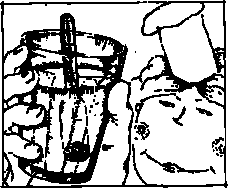
\includegraphics[width=0.55\textwidth]{figures/fig-7-7.pdf}
\caption{Areometer for density measurement.}
\label{fig-7-07}
\end{figure}
Archimedes' principle is valid, of course, for any fluid. If a body of volume $V$ is immersed in a fluid of density $\rho$,
then the weight of the displaced fluid -- and this is just the buoyant force -- will be equal to $\rho gV$.

The working of simple instruments controlling properties of fluid products is based on Archimedes' principle.
If alcohol or milk is diluted in water, its density will change; but it is possible to judge its composition on the
basis of its density. Such a measurement is simply and easily performed with the aid of an areometer \figr{fig-7-07}.

An areometer lowered into a liquid will be immersed to a greater or smaller depth depending on its density. An areometer will be in a state of equilibrium when the buoyant force becomes equal to the weight of the areometer.

Divisions are marked off on an areometer, and the density of a liquid is read from the marking which appears at its surface. Areometers applied for the control of alcohol are called alcoholometers, and those for the control of milk lactometers.

The average density of a person's body is somewhat greater than unity. Anyone unable to swim will drown in fresh water. Salt water has. a density greater than unity. The salinity of the water in most seas is insignificant, and its density, although greater than unity, is less than the average density of the human body. The density of the water in the Bay of Kara-Bogaz-Gol in the Caspian Sea is 1.18. This is greater than the average density of the human body. It is impossible to drown in this bay. One can lie on the water and read a book.

Ice floats on water. The preposition ``on'', incidentally, is somewhat out of place here. The density of ice is about 10\% less than that of water, so it follows from Archimedes' principle that approximately nine-tenth of a piece of ice is submerged in water. It is precisely this circumstance that makes it so dangerous for ocean liners to come across icebergs.

If a balance scale is in equilibrium in air, this does not imply that it will be in equilibrium in a vacuum. Archimedes' principle refers to air to the same degree as to water. A buoyant force equal to the weight of the displaced air acts on a body in air. A body ``weighs'' less in air than in a vacuum. The greater the volume of a body, the greater will be its loss of weight. A ton of
wood loses more weight than a ton of lead. To the humorous question of which is lighter, there is the same kind
of answer: a ton of lead is heavier than a ton of wood if
they are weighed in air.

The loss of weight in air is slight as long as we are considering small bodies. However, in weighing a piece the size of a room, we would ``lose'' several tens of kilograms. For exact weighing, the correction due to the loss of weight of large bodies in air should be taken into account.

The buoyant force in air permits us to construct balloons, aerostats and dirigibles of various types. For this
one must have a gas lighter than air.

If a balloon of volume \SI{1}{\meter\cubed}  is filled with hydrogen, \SI{1}{\meter\cubed} of which has a weight equal to \SI{0.09}{\kgf}, then the lift -- the difference between the buoyant force and the weight of the gas -- will equal
\begin{equation*}%
\SI{1.29}{\kgf} - \SI{0.09}{\kgf} = \SI{1.20}{\kgf}
\end{equation*}
 \SI{1.29}{\kilo\gram\per\centi\metre\cubed} is the density of air.

Hence, a load of about a kilogram can be attached to such a balloon, and this will not prevent it from flying
above the clouds.

It is clear that with relatively small volumes -- of several hundred cubic metres -- hydrogen balloons are capable of raising considerable loads into the air.

A serious defect of hydrogen aerostats is the inflammability of hydrogen. Together with air, hydrogen forms
an explosive mixture. Tragic accidents have marked the history of the creation of aerostats.

Therefore, when helium was discovered, people started filling balloons with it. Helium is twice as heavy as hydrogen and the lift of a balloon filled with it is smaller. But will this difference be significant? The lift of a \SI{1}{\meter\cubed} balloon filled with helium is found as the difference $\SI{1.29}{\kgf} - \SI{0.18}{\kgf} = \SI{1.11}{\kgf}$.
The lift has decreased by only 8\%. At the same time, the advantages of helium are obvious.

The aerostat was the first apparatus with whose aid people rose in the air. Aerostats with a hermetically sealed car have been used up to the present day for investigating the upper layers of the atmosphere. They are called stratospheric balloons. They rise to a height of more than \SI{20}{\kilo\meter}.
\begin{figure}[!ht]
\centering
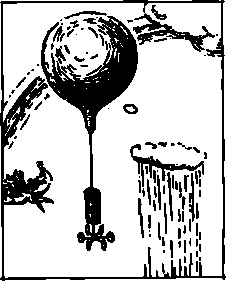
\includegraphics[width=0.55\textwidth]{figures/fig-7-8.pdf}
\caption{A stratospheric balloon for studying upper layers of the atmosphere with various measuring instruments.}
\label{fig-7-08}
\end{figure}
Balloons equipped with various measuring devices and transmitting the results of their measurements by radio \figr{fig-7-08} are widely used at the present time. Such radiosondes contain miniature radio transmitters with batteries which report on the humidity, temperature and atmospheric pressure at various heights by means of prearranged signals.

One can send an unguided aerostat on a long journey and determine rather accurately where it will land. For this it is necessary that the aerostat climb to a great height, of the order of \SIrange{20}{30}{\kilo\meter}. Air currents are extremely stable at such heights, and the path of the aerostat can be calculated quite well beforehand. When necessary, one can automatically change the lift of the aerostat by letting out gas or throwing off ballast. 

Aerostats on which a motor with a propeller was installed were previously used for flights. Such airships were streamlined. Airships lost the competition with airplanes even in comparison with planes of 30 years ago, they are clumsy, difficult to control, move slowly and have a ``low ceiling''. It is believed that airships would be advantageous for carrying cargo.


\section{Extremely Low Pressures. Vacuum}
A vessel which is technically empty still contains an enormous number of molecules.

Molecules of gas constitute a considerable hindrance in many physical instruments. Radio tubes, $X$-ray tubes,
accelerators of elementary particles-all these instruments require a vacuum (derived from the Latin \emph{vacuus}
meaning ``empty''), i.e. space free of gas molecules. There should also be a vacuum in an ordinary electric lamp. If air enters a lamp, it will oxidize and immediately burn out.

In the best vacuum instruments, vacuum of the order of \SI{d-8}{\milli\meter} -\si{\mercury} is produced. A completely negligible pressure, it would seem: the level of mercury in a manometer would move by a hundred-millionth of a millimetre if the pressure changed by such an amount. 

However, there are still several hundred million molecules in \SI{1}{\centi\meter\cubed} at this meagre pressure.

It is interesting to compare the void of interstellar space with such a vacuum -- there one finds an average of one elementary particle of matter in several cubic centimetres.

Special pumps are employed in order to obtain vacuum. An ordinary pump removing gas by means of the motion of a piston can create a vacuum of at best \SI{0.01}{\milli\meter\mercury}. A good or, as one says, high vacuum can be obtained with the aid of a so-called diffusion (mercury or oil) pump in which gas molecules are caught up in a stream of mercury or oil vapour.

Mercury pumps, bearing the name of their inventor, Langmuir, start working only after a preliminary exhaustion to a pressure of about \SI{0.1}{\milli\meter\mercury}; such a preliminary rarefaction is called a forevacuum.

This is the way it works. A small glass container is connected to a vessel with mercury, an evacuated space and a forepump, The mercury is heated and the forepump carries away its vapour. The mercury vapour captures molecules of the gas along the way and brings them to the forepump. The mercury vapour condenses (cooling by means of running water is provided for), and the liquid
trickles down into the vessel from which the mercury began its journey.

A vacuum obtained under laboratory conditions, as we have just said, is still far from empty in the absolute sense of the word. A vacuum is greatly rarefied gas. The properties of such a gas may differ essentially from those of an ordinary gas.

The motion of the molecules ``forming a vacuum'' changes its character when the mean free path of a molecule becomes greater than the dimensions of the vessel containing the gas. The molecules then rarely collide with each other and travel in straight zigzags striking against first one and then another wall of the vessel. We shall speak in detail about the motion of molecules
in the second book. It is known to the reader that mean free path of a molecule in air at atmospheric pressure is equal to \SI{5e-6}{\centi\meter}. If we increase it by a factor of \num{d7}, it will be \SI{50}{\centi\meter}, i.e. will be noticeably greater than an average sized vessel. Since the mean free path is inversely proportional to the density, and hence also to the pressure, the pressure must be \num{d-7} of atmospheric pressure, or approximately \SI{d-4}{\milli\meter\mercury}.

Even interplanetary space is not entirely empty. But the density of the matter in it is about \SI{5e-24}{\gram\per\cubic\centi\metre}.
The main component of interplanetary matter is atomic hydrogen. At the present time, it is considered that cosmic space contains several hydrogen atoms per \SI{1}{\gram\per\centi\metre\cubed}. If a hydrogen molecule were enlarged to the size of a pea and placed in Moscow, its nearest  ``cosmic neighbour'' would prove to be in Tula.

\section{Pressures of Millions of Atmospheres}

We daily come across high pressures exerted on small surfaces. Let us estimate, for example, what the pressure will be at the point of a needle. Assume that the tip of a needle or nail has a linear dimension of \SI{0.1}{\milli\meter}. This implies that the area of the point will be about \SI{0.0001}{\centi\meter\squared}. If a rather modest force of \SI{10}{kgf} acts on such a nail, then the tip of the nail will exert a pressure of \SI{100000}{\atmos}. It's no wonder that the pointed objects so easily penetrate deeply into dense bodies.

It follows from this example that to create high pressures on small surfaces is quite a common thing. The situation is completely different if the question is to create high pressures on large surfaces.

\begin{figure}[!ht]
\centering
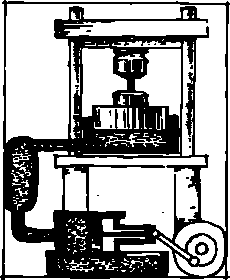
\includegraphics[width=0.4\textwidth]{figures/fig-7-9.pdf}
\caption{Apparatus for creating high pressures.}
\label{fig-7-9}
\end{figure}

The creation of high pressures under laboratory conditions is accomplished with the aid of powerful presses,
for example, hydraulic ones \figr{fig-7-9}. The force of  the press is transmitted to a piston of small area, and
the piston forces its way into the vessel within which we wish to create a high pressure.

Pressures of several thousand atmospheres can be created in this manner without any particular difficulty. But in order to obtain ultrahigh pressures, we must complicate the experiment, since the material composing the vessel cannot withstand such pressures.

Here nature has met us half-way. It turns out that metals become considerably stronger under pressures of the order of \SI{20000}{\atmos}. Therefore, an apparatus for obtaining ultrahigh pressures is submerged in a liquid which is under a pressure of the order of \SI{30000}{\atmos}. In this case, one is able to create pressures of several hundred thousands of atmospheres (but again with
a piston). The highest pressure -- \SI{400000}{\atmos} -- was obtained by the American physicist Percy Williams Bridgman.

Our interest in obtaining ultrahigh pressures is far from idle. Phenomena which are impossible to induce by other methods can occur at such pressures. Artificial diamonds were obtained in 1955. A pressure of \SI{100000}{\atmos} and, in addition, a temperature of \SI{2000}{\kelvin} were required for this. Ultrahigh pressures of the order of \SI{300000}{\atmos} on large surfaces are formed during explosions of solid or liquid explosive materials -- nitroglycerine, trotyl, etc. Incomparably higher pressures attaining \SI{d13}{\atmos} arise, within an atomic bomb during its explosion. Pressures during an explosion exist for a very short time.

There are constant high pressures deep inside celestial bodies including the Earth, of course. The pressure at the centre of the Earth is equal to approximately 3 million atmospheres.
